% Options for packages loaded elsewhere
\PassOptionsToPackage{unicode}{hyperref}
\PassOptionsToPackage{hyphens}{url}
%
\documentclass[
]{article}
\usepackage{amsmath,amssymb}
\usepackage{lmodern}
\usepackage{iftex}
\ifPDFTeX
  \usepackage[T1]{fontenc}
  \usepackage[utf8]{inputenc}
  \usepackage{textcomp} % provide euro and other symbols
\else % if luatex or xetex
  \usepackage{unicode-math}
  \defaultfontfeatures{Scale=MatchLowercase}
  \defaultfontfeatures[\rmfamily]{Ligatures=TeX,Scale=1}
\fi
% Use upquote if available, for straight quotes in verbatim environments
\IfFileExists{upquote.sty}{\usepackage{upquote}}{}
\IfFileExists{microtype.sty}{% use microtype if available
  \usepackage[]{microtype}
  \UseMicrotypeSet[protrusion]{basicmath} % disable protrusion for tt fonts
}{}
\makeatletter
\@ifundefined{KOMAClassName}{% if non-KOMA class
  \IfFileExists{parskip.sty}{%
    \usepackage{parskip}
  }{% else
    \setlength{\parindent}{0pt}
    \setlength{\parskip}{6pt plus 2pt minus 1pt}}
}{% if KOMA class
  \KOMAoptions{parskip=half}}
\makeatother
\usepackage{xcolor}
\usepackage[margin=1in]{geometry}
\usepackage{graphicx}
\makeatletter
\def\maxwidth{\ifdim\Gin@nat@width>\linewidth\linewidth\else\Gin@nat@width\fi}
\def\maxheight{\ifdim\Gin@nat@height>\textheight\textheight\else\Gin@nat@height\fi}
\makeatother
% Scale images if necessary, so that they will not overflow the page
% margins by default, and it is still possible to overwrite the defaults
% using explicit options in \includegraphics[width, height, ...]{}
\setkeys{Gin}{width=\maxwidth,height=\maxheight,keepaspectratio}
% Set default figure placement to htbp
\makeatletter
\def\fps@figure{htbp}
\makeatother
\setlength{\emergencystretch}{3em} % prevent overfull lines
\providecommand{\tightlist}{%
  \setlength{\itemsep}{0pt}\setlength{\parskip}{0pt}}
\setcounter{secnumdepth}{-\maxdimen} % remove section numbering
\newlength{\cslhangindent}
\setlength{\cslhangindent}{1.5em}
\newlength{\csllabelwidth}
\setlength{\csllabelwidth}{3em}
\newlength{\cslentryspacingunit} % times entry-spacing
\setlength{\cslentryspacingunit}{\parskip}
\newenvironment{CSLReferences}[2] % #1 hanging-ident, #2 entry spacing
 {% don't indent paragraphs
  \setlength{\parindent}{0pt}
  % turn on hanging indent if param 1 is 1
  \ifodd #1
  \let\oldpar\par
  \def\par{\hangindent=\cslhangindent\oldpar}
  \fi
  % set entry spacing
  \setlength{\parskip}{#2\cslentryspacingunit}
 }%
 {}
\usepackage{calc}
\newcommand{\CSLBlock}[1]{#1\hfill\break}
\newcommand{\CSLLeftMargin}[1]{\parbox[t]{\csllabelwidth}{#1}}
\newcommand{\CSLRightInline}[1]{\parbox[t]{\linewidth - \csllabelwidth}{#1}\break}
\newcommand{\CSLIndent}[1]{\hspace{\cslhangindent}#1}
\ifLuaTeX
  \usepackage{selnolig}  % disable illegal ligatures
\fi
\IfFileExists{bookmark.sty}{\usepackage{bookmark}}{\usepackage{hyperref}}
\IfFileExists{xurl.sty}{\usepackage{xurl}}{} % add URL line breaks if available
\urlstyle{same} % disable monospaced font for URLs
\hypersetup{
  pdftitle={Diamonds},
  pdfauthor={Stuart Leeds},
  hidelinks,
  pdfcreator={LaTeX via pandoc}}

\title{Diamonds}
\author{Stuart Leeds}
\date{19/03/2022}

\begin{document}
\maketitle

\hypertarget{introduction}{%
\section{Introduction}\label{introduction}}

Are diamonds really a girls best friend? Are they even forever? They are
certainly expensive; and they last a long time. Diamonds are the hardest
known natural material and are developed deep underground over millennia
of immense pressure and temperature. See the
\href{https://en.wikipedia.org/w/index.php?title=Diamond\&oldid=1073530080}{\emph{Wikipedia}}
entry for general information about diamonds.

The purpose of this short article is to analyse a dataset of diamond
information using various \texttt{R} packages. We are interested in the
descriptive statistics of the dataset; the correlation between price and
the main variables; and whether the relationship between carat and the
price of diamonds is mediated by cut, color and clarity.

\hypertarget{data}{%
\section{Data}\label{data}}

The \texttt{diamonds} data are found in \texttt{ggplot2}
(\protect\hyperlink{ref-R-ggplot2}{Wickham et al., 2022}) and consist of
almost 54,000 round-cut diamonds with the following variables:

\begin{quote}
\begin{enumerate}
\def\labelenumi{\arabic{enumi}.}
\item
  \textbf{Carat} \emph{(weight of the diamond):} 0.2 to 5.01ct.
\item
  \textbf{Cut} \emph{(quality of the cut):} Fair, Good, Very Good,
  Premium, Ideal.
\item
  \textbf{Color:} {[}Best{]} D, E, F, G, H, I, J {[}Worst{]}.
\item
  \textbf{Clarity} \emph{(how clear the diamond is):} {[}Worst{]} I1,
  SI2, SI1, VS2, VS1, VVS2, VVS1, IF {[}Best{]}.
\item
  \textbf{Depth} \emph{(total depth percentage):} 43 to 79\%, calculated
  with either
  \[\frac{z}{mean(x, y)}\times 100 \quad \text{or}\quad \frac{2
  \times z}{(x + y)}\times 100\]
\item
  \textbf{Table} \emph{(width of top of diamond relative to widest point
  {[}percentage of diameter{]}):} 43 to 95\%.
\item
  \textbf{Price} \emph{(US\$):} 326 to 18823.

  The variables below are used to calculate \emph{Depth (Item 5)}, and
  are not used in any analysis in this article:\\
  \textbf{x} \emph{(length):} 0 to 10.74mm.\\
  \textbf{y} \emph{(width):} 0 to 58.9mm.\\
  \textbf{z} \emph{(depth):} 0 to 31.8mm.
\end{enumerate}

\emph{information from \texttt{?diamonds}}.
\end{quote}

\begin{table}
\caption{\label{tab:tables}<b>Table 1.</b><br><i>Number of Occurances and Average Price for each Categorical Variable</i>}
\begin{table}

\centering
\begin{tabular}[t]{lrr}
\toprule
\multicolumn{1}{l}{\$Cut\$} & \multicolumn{1}{l}{\$Color\$} & \multicolumn{1}{l}{\$Clarity\$} \\
\cmidrule(l{3pt}r{3pt}){1-1} \cmidrule(l{3pt}r{3pt}){2-2} \cmidrule(l{3pt}r{3pt}){3-3}
 & N & Avg Price\\
\midrule
Fair & 1,610 & 4,358.76\\
Good & 4,906 & 3,928.86\\
Very Good & 12,082 & 3,981.76\\
Premium & 13,791 & 4,584.26\\
Ideal & 21,551 & 3,457.54\\
\bottomrule
\multicolumn{3}{l}{\rule{0pt}{1em}\textit{\$Notes.\$ }}\\
\multicolumn{3}{l}{\rule{0pt}{1em}Color- D (Absolutely colorless or icy-white); E \& F (Colorless); G - J (Near colorless).}\\
\multicolumn{3}{l}{\rule{0pt}{1em}Clarity- [FL (Flawless), not listed here]; IF (Internally flawless); VVS1 \& VVS2 (Very very slightly included); VS1 \& VS2 (Very slightly included); SI1 \& SI2 (Slightly included); I1 - I3 (Included).}\\
\multicolumn{3}{l}{\rule{0pt}{1em}See Brilliant Earth for further details of variable identification (ID) categories: [\$Cut\$](https://www.brilliantearth.com/diamond-cuts/); [\$Color\$](https://www.brilliantearth.com/diamond-color/); [\$Clarity\$](https://www.brilliantearth.com/diamond-clarity/)}\\
\end{tabular}
\end{table}\begin{table}

\centering
\begin{tabular}[t]{lrr}
\toprule
 & N & Avg Price\\
\midrule
D & 6,775 & 3,169.95\\
E & 9,797 & 3,076.75\\
F & 9,542 & 3,724.89\\
G & 11,292 & 3,999.14\\
H & 8,304 & 4,486.67\\
\addlinespace
I & 5,422 & 5,091.87\\
J & 2,808 & 5,323.82\\
\bottomrule
\end{tabular}
\end{table}\begin{table}

\centering
\begin{tabular}[t]{lrr}
\toprule
 & N & Avg Price\\
\midrule
I1 & 741 & 3,924.17\\
SI2 & 9,194 & 5,063.03\\
SI1 & 13,065 & 3,996.00\\
VS2 & 12,258 & 3,924.99\\
VS1 & 8,171 & 3,839.46\\
\addlinespace
VVS2 & 5,066 & 3,283.74\\
VVS1 & 3,655 & 2,523.11\\
IF & 1,790 & 2,864.84\\
\bottomrule
\end{tabular}
\end{table}
\end{table}

\hfill\break

\begin{figure}

{\centering 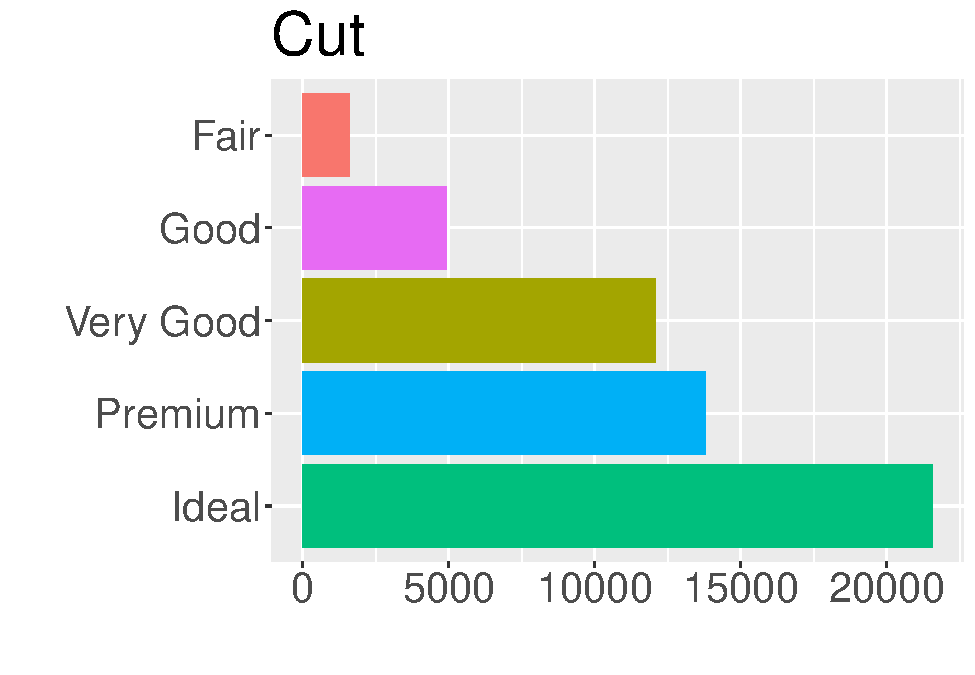
\includegraphics[width=0.333\linewidth]{diamonds_files/figure-latex/show categorical figures-1} 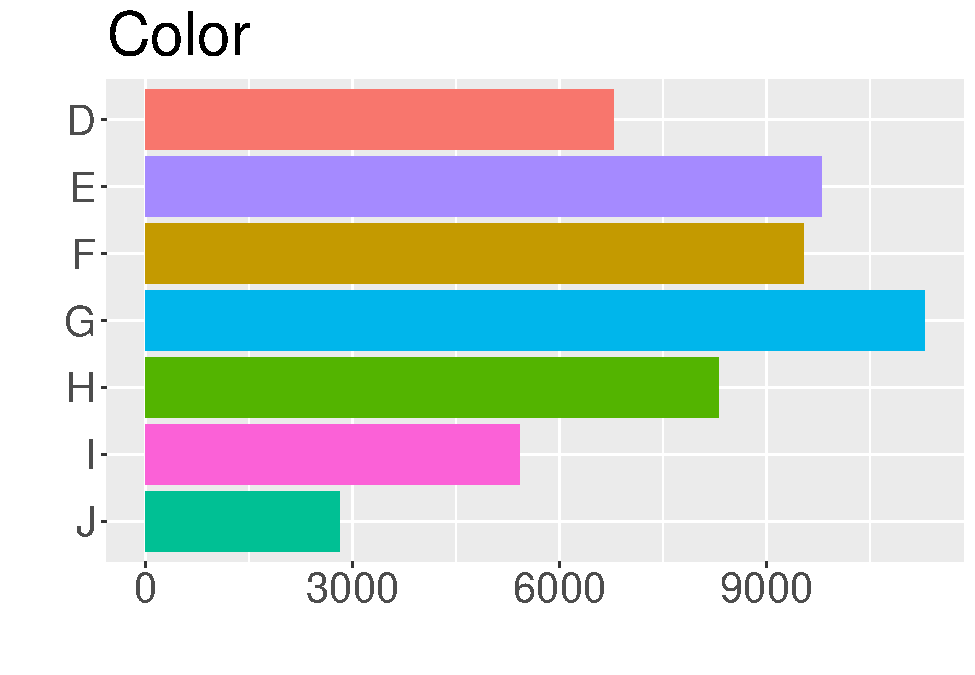
\includegraphics[width=0.333\linewidth]{diamonds_files/figure-latex/show categorical figures-2} 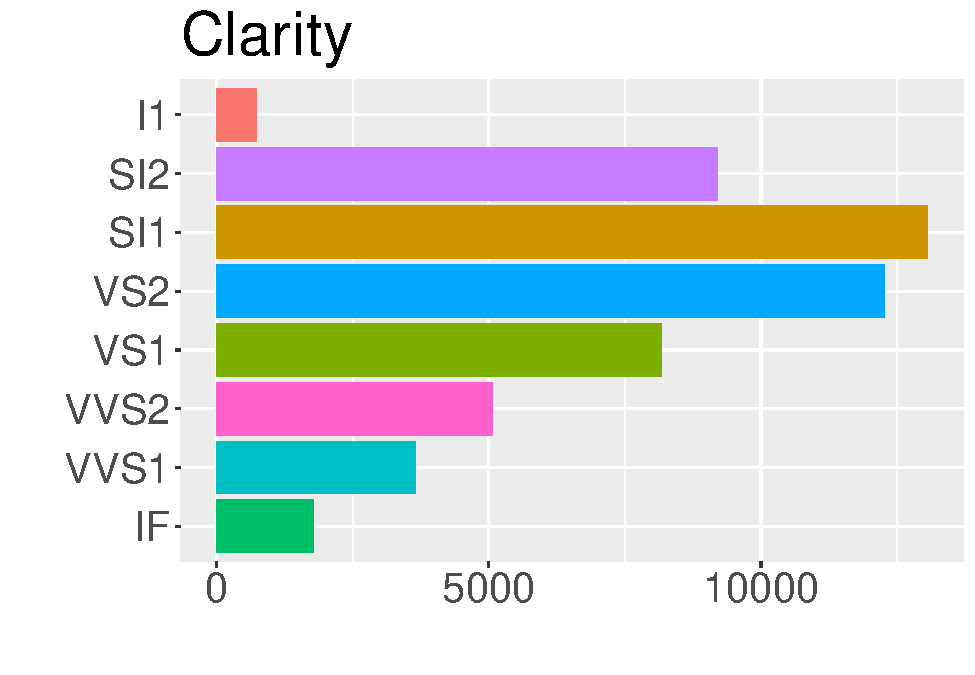
\includegraphics[width=0.333\linewidth]{diamonds_files/figure-latex/show categorical figures-3} 

}

\caption{__Figure 1.__ _Graphical Representation of Number of Occurances for each Categorical Variable_}\label{fig:show categorical figures}
\end{figure}

\hypertarget{method}{%
\section{Method}\label{method}}

\hypertarget{results}{%
\section{Results}\label{results}}

\textbf{Correlation}

Correlational analysis shows the relationships between variables whether
significant, or otherwise (see Figure 2). As expected all the main
variables in the diamond data set are significantly correlated with
price. Of the significant positive relationships, \emph{carat} is the
strongest (\(r=\) \(0.92\), \(p< .001\)), with weak correlations with
price found for \emph{color} (\(r=\) \(0.17\), \(p< .001\)). The
remaining variables have negative, weak, yet significant correlations
with price: \emph{cut} (\(r=\) \(-0.15\), \(p< .001\)) and
\emph{clarity} (\(r=\) \(-0.05\), \(p< .001\)).

The variance of each correlation with price can be explained with
\(r^2\). For example, \(85\%\) of the variance in the price of diamonds
can be explained by \emph{carat} (\(r^2=\) \(0.85\)). The same principle
applies to the other correlations: \emph{cut} (\(r^2=\) \(0.022\))
explains \(2.2\%\) of the variance in price); \emph{color} (\(r^2=\)
\(0.03\); \(3\%\)); and \emph{clarity} (\(r^2=\) \(0.003\); \(0.3\%\)).

\begin{figure}

{\centering 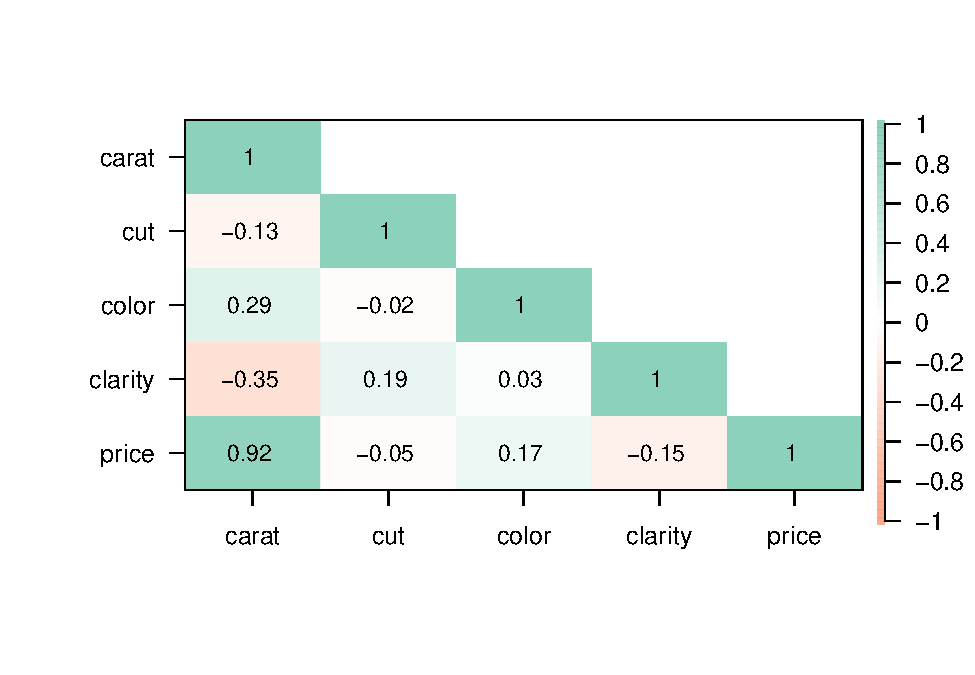
\includegraphics{diamonds_files/figure-latex/corr plot-1} 

}

\caption{__Figure 2.__ _Correlation Plot of Diamonds Data with the Main Variables_}\label{fig:corr plot}
\end{figure}

\hfill\break
\textbf{Linear Regression and Mediation}

\begin{table}

\caption{\label{tab:lr table}<b>Table 2.</b><br><i>Linear Regression Showing the Effect Size Between Variables and Price.</i>}
\centering
\begin{tabular}[t]{llllll}
\toprule
\$Predictor\$ & \$b\$ & \$95\textbackslash{}\% \textbackslash{}space CI\$ & \$t\$ & \$\textbackslash{}mathit\{df\}\$ & \$p\$\\
\midrule
Intercept & -4,661.17 & {}[-4,715.25, -4,607.10] & -168.94 & 53935 & < .001\\
Carat & 8,783.77 & {}[8,758.90, 8,808.65] & 692.09 & 53935 & < .001\\
Cut & 155.70 & {}[146.17, 165.23] & 32.01 & 53935 & < .001\\
Color & -319.67 & {}[-326.14, -313.20] & -96.81 & 53935 & < .001\\
Clarity & 524.84 & {}[517.93, 531.76] & 148.80 & 53935 & < .001\\
\bottomrule
\end{tabular}
\end{table}

\begin{figure}

{\centering 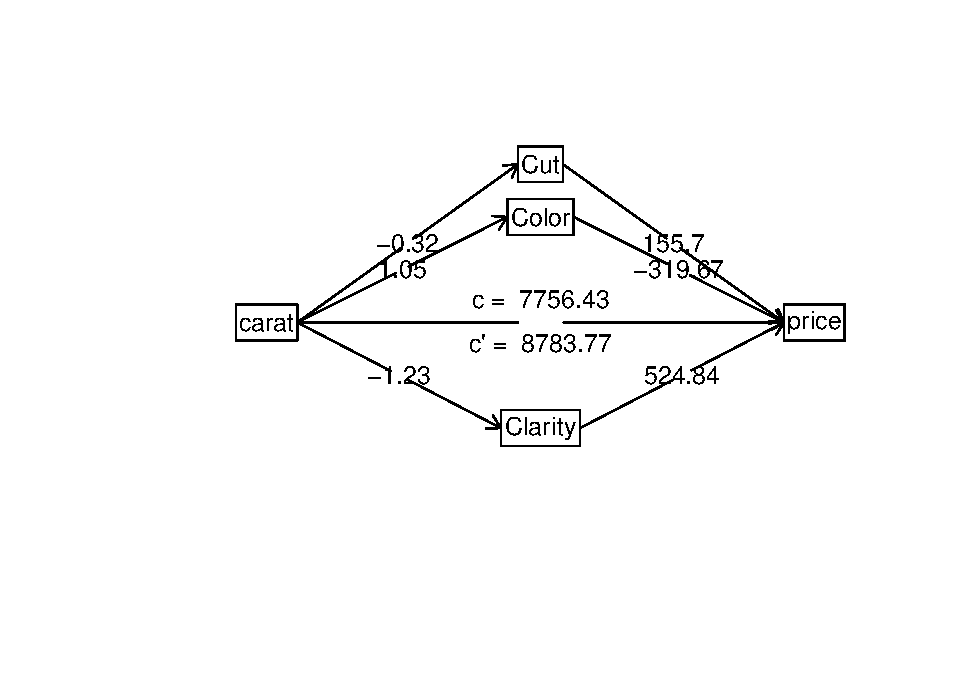
\includegraphics{diamonds_files/figure-latex/med calc-1} 

}

\caption{__Figure 3.__ _Mediation Plot Between Carat and Price Mediated by Cut, Color and Clarity_}\label{fig:med calc}
\end{figure}

\begin{figure}

{\centering \includegraphics[width=0.5\linewidth]{diamonds_files/figure-latex/correlation venns-1} 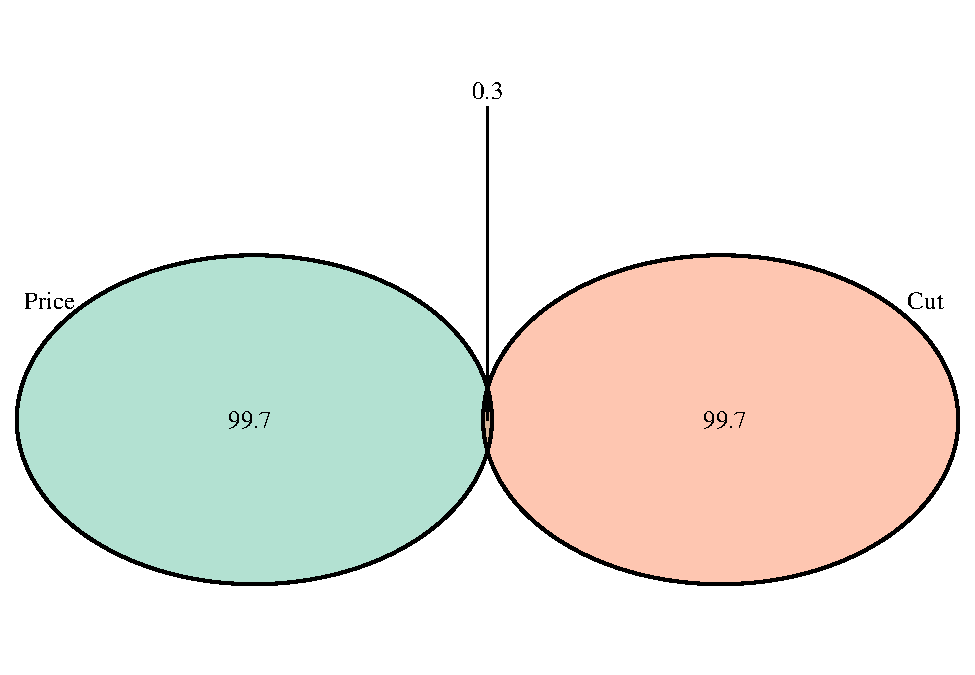
\includegraphics[width=0.5\linewidth]{diamonds_files/figure-latex/correlation venns-2} 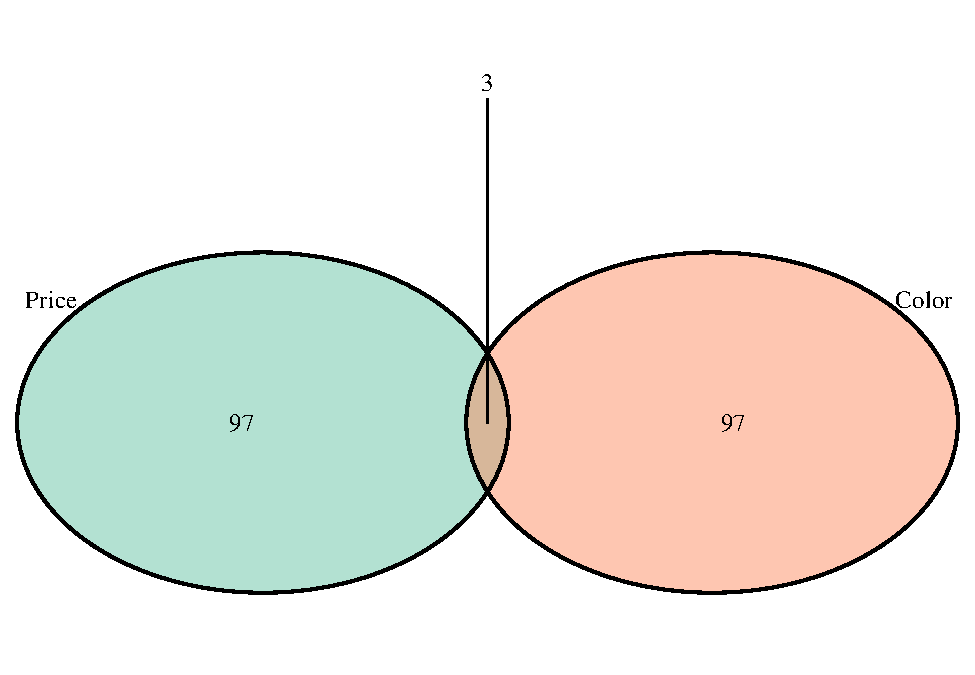
\includegraphics[width=0.5\linewidth]{diamonds_files/figure-latex/correlation venns-3} 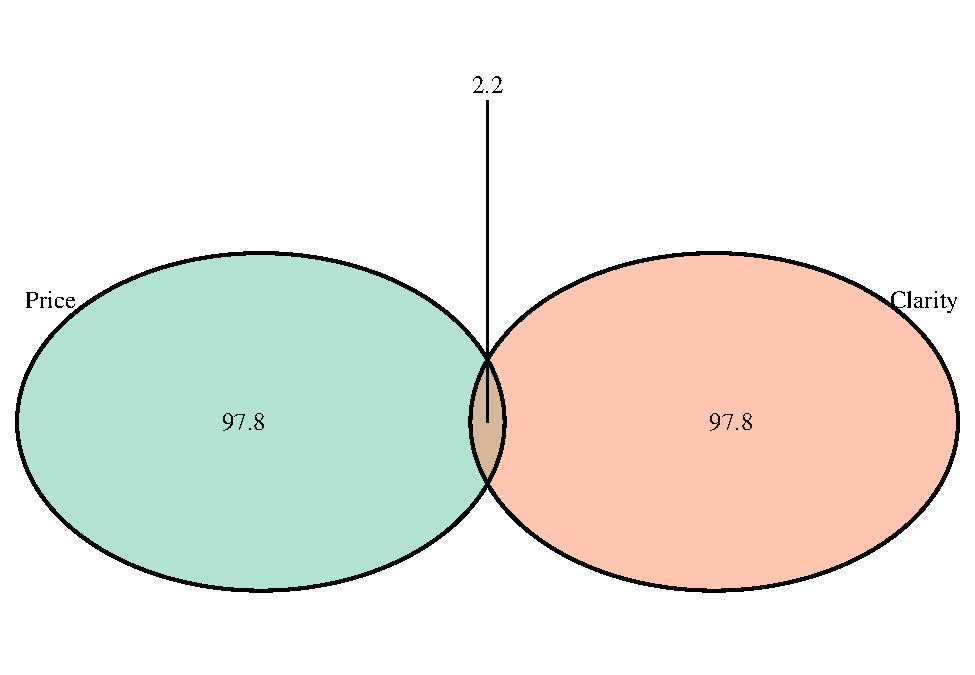
\includegraphics[width=0.5\linewidth]{diamonds_files/figure-latex/correlation venns-4} 

}

\caption{__Figure 4.__ _Graphical Representation of Corrrelations_}\label{fig:correlation venns}
\end{figure}

\hfill\break
\textbf{Discussion}

\hfill\break
\textbf{Conclusion}

\textbf{References}

\hypertarget{refs}{}
\begin{CSLReferences}{1}{0}
\leavevmode\vadjust pre{\hypertarget{ref-R-ggplot2}{}}%
Wickham, H., Chang, W., Henry, L., Pedersen, T. L., Takahashi, K.,
Wilke, C., Woo, K., Yutani, H., \& Dunnington, D. (2022). \emph{ggplot2:
Create elegant data visualisations using the grammar of graphics}.
\url{https://CRAN.R-project.org/package=ggplot2}

\end{CSLReferences}

\hfill\break

\end{document}
